% latex

% title: SwipProteomics
% author twab
% description: response to reviewers

\documentclass[12pt]{article}

\usepackage{amsmath}
\usepackage{amssymb}
\usepackage{amsthm}
\usepackage{caption}
\usepackage{changepage}
\usepackage{fancyhdr}
\usepackage{graphicx}
\usepackage{tikz}
\usepackage{titlesec}
\usepackage[margin=1.0in]{geometry}
\usepackage{inconsolata} % for mono font \texttt

\pagestyle{fancy}
\pagenumbering{gobble} 
\setlength\parindent{0pt}
\graphicspath{ {./figs/} }

\lhead{Tyler W. A. Bradshaw}
\rhead{Response to eLife Reviewers} 


\begin{document}

\section{Reanalysis TMT Proteomics Data}

At the center of the cogent critique of our manuscript 
was the questioned statistical validity of our previously described approach.   
Succinctly, the issue at question is whether or not the R package \texttt{edgeR}
is an appropriate tool for analysis of protein mass spectrometry data.\\

Statistical inference in \texttt{edgeR} is built on a 
negative binomial (NB), generalized linear model (GLM) framework. 
Therefore, the data are assumed to be adequately described by a NB distribution 
parameterized by a dispersion parameter, $\phi$. \footnotemark{} \\

\footnotetext{ The dispersion parameter can take several forms. 
\texttt{edgeR} supports three dispersion models: 'common', 'trended', and 
'tagwise'. However, when using \texttt{edgeR's} 
robust quasi-likelihood test methods, only global (i.e. 'common' or 'trended') 
dispersion metrics are appropriate (see ?\texttt{edgeR::glmQLFit}).}

Previously we used a customized workflow \footnotemark{} to preprocess
and normalize the data prior to performing statistical testing using
\texttt{edgeR's} flexible GLM framework. However, we failed to thoughougly
consider the overall adequacy of the NB framework for mass spectrometry data. 
Here we reconsider its appropriatness for our TMT proteomics dataset.  \\

\footnotetext{ The most important step in our normalization approach is 
IRS normalization. MS2 random sampling results in identification and
quantification of proteins by different peptides in each MS experiment.
To account for this source of variability, protein measurements are adjusted by
a scaling factor such that the geometric mean of all internal reference
standards are equal (Plubell et al., 2017).
This is essential to account for the stochasticisity of peptide
quantification in MS experiments. Phillip Wilmarth's GitHub offers an 
excellent exploration of IRS normalization.
}

We evaluated the overall adequacy of the \texttt{edgeR} model by plotting the 
residual deviance of all proteins against their theoretical, 
normal quantiles in a quantile-quantile plot. \textbf{Figure \ref{fig:gof}} 
illustrates the overall lack of fit for the three disperion models fit by 
\texttt{edgeR}.  As an alternative to \texttt{edgeR} we considered 
\texttt{MSstatsTMT}, an extension of MSstats for analysis of TMT proteomics
experiments. \\

\texttt{MSstatsTMT} utilizes a linear mixed-model framework. The strength of 
linear mixed models is thier ability to account for complex sources of variation 
in an experimental design. In mixed models, one or more covariates are a 
categorical variable representing representing experimentaal or observational 
"units" in the data set (Bates 2010). \\

A TMT proteomics experiment consists of \texttt{m = 1...M} concatensions of 
isobaric TMT-labeled samples or \texttt{Mixtures}. 
Each TMT channel is dedicated to the analysis of \texttt{c = 1...C}
individual biological or treatment \texttt{Conditions} prepared from one
\texttt{b = 1...B} biological replicates or \texttt{Subjects}. 
A single mixture may be profiled in \texttt{t = 1...T} technical replicate 
mass spectrometry runs. Each protein is measured \texttt{M x C x B x T} times.\\

The full linear mixed model describing such an experiment is of the form:

\begin{equation} \label{eq1}
	Y_{mcbt} = \mu + Mixture_m + TechRepMixture_{t(m)} + Condition_c + 
	Subject_{mcb} + \epsilon_{mcbt}
\end{equation}

\begin{gather*}
	Condition_c = \sum_{C=1}^{C} \\
	Mixture_m \sim N(0,\sigma^2_M) \\
	Subject_mcb \sim N(0,\sigma^2_M) \\
	TechRepMixture \sim N(0, \sigma^2_T) \\
	\epsilon_{mcbt} \sim N(0,\sigma^2) \\
\end{gather*}

In an experiment with multiple mixtures and biological replicates, but no
technical replication of mixture (T = 1) \texttt{MSstatsTMT} fits the model:
Where Mixture is a mixed-effect and quantifies variation between TMT mixtures.
Condition is a fixed effect (mean = 0) and in our experiment represents the
interaction of terms \texttt{Genotype} and \texttt{BioFraction}. $\epsilon$ 
is a random effect representing both biological and technical variation, 
quantifying any remaining error. \\

If a term is not estimable, then it is removed from the model. In our
experimental design, we made measurments from seven  biological subcelluular
fractions (BioFractions) from each subject. Thus, we should include the term 
Subject, representing the 6 individual mice or subjects analyzed in our 
experiment. However, in our design \texttt{Mixture} is confounded with the
term \texttt{Subject} -- in each mixture we analyzed all \texttt{BioFractions} 
from a single Control and Mutant mouse. Thus we can choose to account for the 
effect of \texttt{Mixture} or \texttt{Subject}, but not both. 
Assuming Mixture contributes greater to the variance, we drop the term Subject,
and the reduced model is equivalent  to \ref{eq1}. \\

For experiments with multiple mixtures and biological replicates, the reduced
model is then:

\begin{equation} \label{eq1}
	Y_{mcbt} = \mu + Mixture_m + Condition_c + \epsilon_{mcb}
\end{equation}

Where Condition is the interaction of Genotype and BioFraction, the 14
combinations of 7 subcellular fractions measured in Control and Mutant mice.

Model based testing of differential abundance between pairs of conditions
is assessed through contrast of conditioned means estimated by fitting the
parameters of the model by REML to obtain $\hat{\beta}$, $\sigma^2$ and
$\hat{V}$.


The degrees of freedome are determined by the Satterthwaite approximation[REF],
and the T-statistic for the contrast is taken to be (lmerTest ref): \\

\begin{equation}
	t = \frac{l^T * \hat{\beta}}{sqrt(l * s^2 * \hat{V} * l^T)}
\end{equation}

$\sigma^2$ is the error from \textbf{Equation} \ref{eq1}.
\(l^T = \sum_{C=1}^{C}=0\) a vector specifying a contrast between positive and 
negative coefficients in the model.

Together the denominator \(sqrt(l * s^2 * \hat{V} * l^T)\) is the standard error
of the contrast computed from the unscaled variance-covariance matrix, $\hat{V}$.


%% figures

\begin{figure}[]
	\begin{center}
		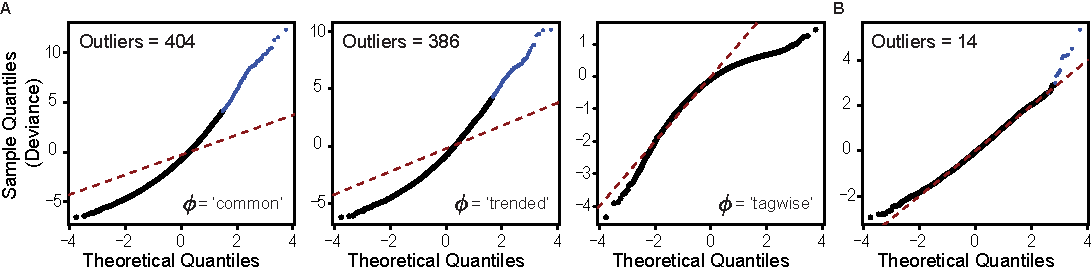
\includegraphics{gof}
		\caption{\textbf{Goodness-of-fit of \texttt{edgeR} (A), and 
		\texttt{MSstats} (B) statistical approaches.} The overall
		adequacy of the linear models fit to the data were assessed 
		by plotting the residual deviance for all proteins as a 
		quantile-quantile plot (McCarthy \textit{et al.}, (2012)). 
		\textbf{(A)} The normalized
		protein data were fit with a NB GLM of the form: 
		\textasciitilde{} \texttt{Mixture + Condition}.
		Where \texttt{Mixure} is a blocking factor that accounts for
		sources of variablity between experiments. Protein-wise deviance
		statistics were transformed to normality and plotted aganis
		theoretical normal quantiles using \texttt{edgeR::gof}.
		\textbf{(B)}
		The normalized protein data were fit with a linear mixed-effects 
		model (LMM) of the form: 
		\texttt{Abundance}
		\textasciitilde{}\texttt{0 + Condition + (1|Mixture)}. 
		Where \texttt{Mixture} indicates the random effect
		of \texttt{Mixture}. The residual deviance and degrees of 
		freedom were extracted from the fitted models, z-score
		normalized, and plotted as in (A). Proteins with significantly 
		poor fit are indicated as outliers in blue 
		(Holm-adjusted P-value $<$ 0.05).}
		\label{fig:gof}
	\end{center}
\end{figure}


\begin{figure}[]
	\begin{center}
		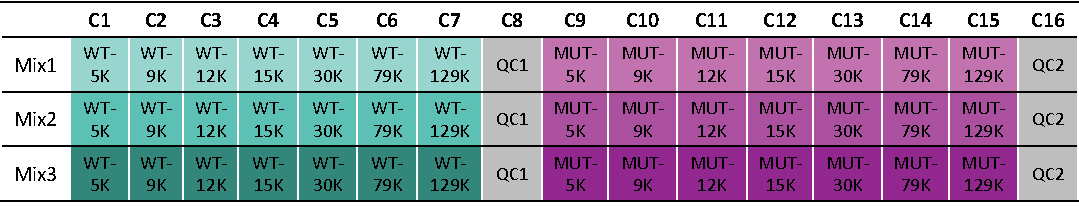
\includegraphics{design}
		\caption{\textbf{Experimental Design}}
		\label{fig:design}
	\end{center}
\end{figure}

\begin{figure}[]
	\begin{center}
		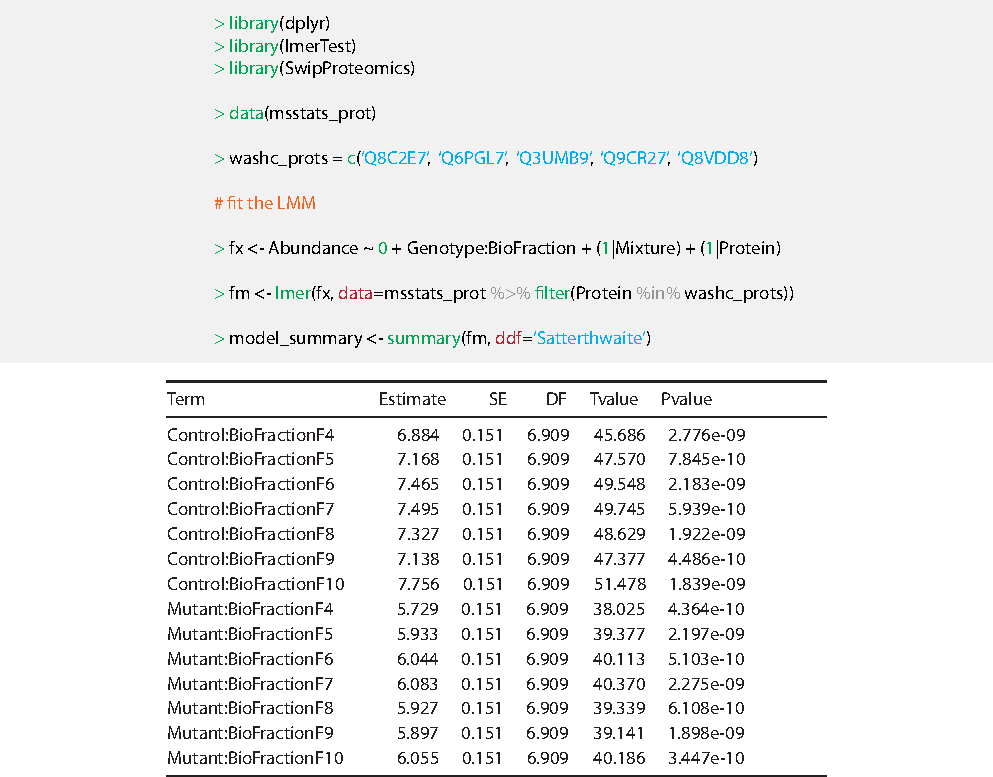
\includegraphics{fit}
		\caption{\textbf{Example: Fit lmer to Wash complex.}}
		\label{fig:design}
	\end{center}
\end{figure}

\begin{figure}[]
	\begin{center}
		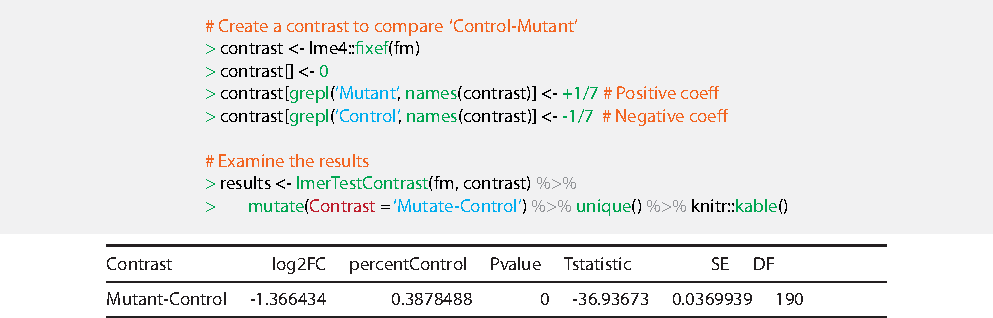
\includegraphics{res1}
		\caption{\textbf{Test for 'Mutant-Control' contrast for
		difference between means of WASH complex proteins..}}
		\label{fig:design}
	\end{center}
\end{figure}


\end{document}
